In this chapter the basic concepts of process mining, text mining, supervised learning and long short-term memory networks are presented. Furthermore, necessary formal definitions and notations are introduced.

\section{Processes and Process Mining}

\begin{definition}[Process]
	A \textit{process} is a collection of activities that are performed in a specific order to achieve a goal.
	A single execution of a process is a \textit{case} or \textit{process instance}, which is identified by a case ID.
\end{definition}

Each performed activity belongs to specific case and is completed at a certain time \cite{DBLP:conf/bpm/AalstAM11}.
For example, a case can be a patient treated in a hospital, a customer journey or an online order.
The time on which an activity for a certain case is performed is specified by a timestamp.
The associated case ID, the performed activity and the timestamp form together an \textit{event}.
An event can have any number of additional attributes, e.g. an attribute describing the resource that carries out the activity.
\begin{table}[htbp!]
	\small
	\setlength\tabcolsep{3pt}
	\begin{tabularx}{\textwidth}{lllllp{4.7cm}l}
		\toprule
		\textbf{ID} & \textbf{Activity}          & \textbf{Timestamp} & \textbf{Resource} & \textbf{Costs} & \textbf{Comment}  \\
		\midrule
		0                & Register patient           & 2020-02-01 14:12   & SYSTEM            & 0             & -     \\
		& Consultation               & 2020-02-01 14:34   & J. Brown, MD    & 24.32         & The patient reports persistent nausea.   \\
		& Blood test                 & 2020-02-01 15:12   & K. Smith         & 14:23         & Test: Complete blood count    \\
		& Evaluate test  & 2020-02-01 16:35   & J. Brown, MD    & 38.67         &No abnormalities in the complete blood count.   \\
		& Release patient            & 2020-02-01 17:24   & SYSTEM            & 0             & -  \\
		&                            &                    &                   &               &     \\
		\midrule
		1                & Register patient           & 2020-02-02 08:20   & SYSTEM            & 0             & -  \\
		& Consultation               & 2020-02-02 14:12   & J. Simpson, MD  & 24.32         & Noticeable tachycardia. No chronic pre-existing conditions are known.    \\
		& MRI & 2020-02-02 16:10   & S. Taylor, MD   & 352.87        & -    \\
		& Release patient            & 2020-02-02 18:33   & SYSTEM            & 0             & -   \\
		&                            &                    &                   &               &     \\
		\midrule
		2                & Register patient           & 2020-02-02 09:08   & SYSTEM            & 0             & -    \\
		& Consultation               & 2020-02-02 09:14   & J. Simpson, MD  & 24.32         & The patient has severe leg injuries due to a motorcycle accident.  \\
		& Hospitalization       & 2020-02-02 09:20   & M. Johnson      & 130.37        & -     \\
		...              & ...                        & ...                & ...               & ...           & ...     \\ \bottomrule
	\end{tabularx}
	\caption[Artificial event log of patient treatments in a hospital]{An artificial event log of patient treatments in a hospital. Each row corresponds to one event. The events are grouped by their case IDs, each representing a single patient.}
	\label{tab:event-log}
\end{table}

If the execution of a business process is logged by an information system, the resulting event data is called \textit{event log}.
Depending on the format of the event log, it can also contain additional data on case level.
Typical formats for event logs, are comma-separated values (CSV) and eXtensible Event Stream (XES) \cite{DBLP:conf/caise/VerbeekBDA10a}, which can be extracted from databases of process-aware information systems.
A table-based representation of an artificial event log describing patient treatments in a hospital can be seen in Table \ref{tab:event-log}.
Besides the case ID, activity and timestamp, the event log also contains information about the identity of the person executing the activity, the costs of the activity and a text comment as an example for a categorical, numerical and textual attribute.

\textit{Process mining} is the discipline that covers all approaches aiming to generate value out of event data.
As an umbrella term, process mining includes or utilizes concepts of business process management, data mining, business process intelligence, big data, workflow management, business process monitoring \cite{DBLP:books/sp/Aalst16} as well as machine learning \cite{DBLP:conf/bpm/VeitGMHT17}.

Traditionally, process mining is divided into a set of subdisciplines; mainly, process discovery, conformance checking, process enhancement and process analytics \cite{DBLP:conf/caise/EckLLA15}.
Process discovery aims to generate process models out of event data in order to understand the control flow of a process and enable further analysis.
Conformance checking is about comparing the intended and observed behavior of a process and identifying deviations.
On top of these diagnostic approaches, process enhancement deals with the improvement of processes regarding compliance, performance and complexity.

Finally, process analytics focuses on the metric and performance evaluation of processes. Similar to conformance checking, this term is closely related to business process monitoring, a rising subfield enabling the analysis of running business processes in real-time.
Driven by the fast and ongoing development of quantitative prediction methods in data science and machine learning, prediction-based methods have also been applied to event data.
These methods add the forward perspective to business process monitoring and deal with forecasting the future of a running process instance, which is also the main focus of this work.


\section{Basic Notations and Sequences}

The set $\mathbb{N}$ denotes the set of all natural numbers $\{1, 2, 3, \dots\}$ and $\mathbb{N}_0 = \mathbb{N} \cup \{0\}$ denotes the set of natural numbers including 0.
The subset of natural numbers up to number $n$ is noted as $[n] = \{1, 2, \dots, n\} \subset \mathbb{N}$ with [0] = $\emptyset$.
\begin{definition}[Sequence]
		A \textit{sequence} of length $n \in \mathbb{N}_0$ over a set $A$ is an ordered collection of elements defined by a function $\sigma \colon [n]\to A$, which assigns each index an element of $A$.
\end{definition}
A sequence  of length $n$ is represented explicitly as $\sigma = \langle a_1, a_2, \dots, a_n\rangle $ with $a_i \in A$ for $1 \leq i \leq n$. In addition, $\langle~\rangle$ is the empty sequence of length $0$.
Given a set $A$, $A^*$ describes the set of all sequences over $A$.
%The set $A^0$ is defined as $\{\langle~\rangle\}$, the set that only contains the empty sequence.
%$A^* = \bigcup\limits_{i\in \mathbb{N}_0} A^i$ is the set of all sequences over $A$ and $A^+ = \bigcup\limits_{i\in \mathbb{N}} A^i = A^* \setminus \{ \langle~\rangle\}$ is the set of all sequences over $A$ with a length of at least 1.
%The concatenation of sequences $\sigma_1$ and $\sigma_2$ is denoted by $\sigma_1 \cdot \sigma_2$.
Moreover, the $i$-th element of a sequence $\sigma = \langle a_1, a_2, \dots, a_n\rangle$ is accessed using $\sigma(i)= a_i$ for $1 \leq i \leq n$.
The length of a sequence is denoted by $|\sigma|$.
For a sequence $\sigma=\langle a_1, a_2, \dots, a_n\rangle$, the function
$hd^k(\sigma)= \langle a_1, a_2, \dots, a_k\rangle$ gives the head or prefix of length $k$ of $\sigma$ for $0 \leq k \leq n$.
% and $tl^k(\sigma)= \langle a_{k+1}, a_{k+2}, \dots, a_n\rangle$ the tail or suffix of length $n-k$ for $0 \leq k \leq n$.
%Note that $\sigma = hd^k(\sigma) \cdot tl^{k}(\sigma)$ for $0 \leq k \leq n$ and any sequence $\sigma$.

A function $f \colon A \to B$ can be lifted element-wise to sequences over $A$, precisely:
\begin{equation*}
f(\sigma) =
\begin{cases}
\langle~\rangle & \text{if $\sigma = \langle~\rangle$} \\
\langle f(a_1), f(a_2), \dots, f(a_n)\rangle & \text{else} 
\end{cases}
\end{equation*}
If an element $a \in A$ appears in a sequence $\sigma \in A^*$, the set membership notation $a \in \sigma$ is used for simplification, i.e. $a \in \sigma = \langle a_1, a_2, \dots a_n \rangle \iff \exists_{1 \leq i \leq n} \colon a = a_i$.

\section{Events, Traces, Event Logs}

Based on the definition of sequences, the concepts of events, traces and event logs can be formalized.
\begin{definition}[Event]
An  \textit{event} is a tuple $e = (c,a,t,d_1,\dots, d_m) \in \mathcal{C} \times \mathcal{A}  \times \mathcal{T} \times \mathcal{D}_1 \times \dots \times \mathcal{D}_m =  \mathcal{E}$ where  $c \in \mathcal{C} $ is the case ID, $a \in \mathcal{A}$ is the executed activity and $t \in \mathcal{T}$ is the timestamp of the event.
The set of possible timestamps is required to be totally ordered by some relation $\leq$.
Furthermore, each event contains a fixed number $m \in \mathbb{N}_0$ of additional attributes $d_1, \dots, d_m$ in their corresponding domains $\mathcal{D}_1, \dots , \mathcal{D}_m$.
In case that no additional attribute data is available ($m = 0$) the event space $\mathcal{E}$ (set of all possible events) is reduced to its minimal form $\mathcal{C} \times \mathcal{A}  \times \mathcal{T}$.
\end{definition}
Each attribute $d \in \mathcal{D}$ of an event (including activity, timestamp and case ID) can be accessed by a corresponding projection function $\pi_D \colon \mathcal{E} \to \mathcal{D}$.
For example, the activity $a$ of an event $e$ is retrieved by $\pi_\mathcal{A}(e) = a$.

Throughout this thesis,  $\mathcal{C} = \mathbb{N}_0$, $|\mathcal{A}| < \infty$ and $ \mathcal{T} = \mathbb{R}$ is assumed, where $t \in \mathcal{T}$ is given in Unix time, precisely the number of seconds since 00:00:00 UTC on 1 January 1970 minus the applied leap seconds.
Each additional attribute is assumed to be numerical, categorical or textual, i.e. $\mathcal{D}_i = \mathbb{R}$, $|\mathcal{D}_i| < \infty$ or $\mathcal{D}_i = \Sigma^\ast$  for $1 \leq i \leq m$ and some fixed language-dependent alphabet $\Sigma$.
\begin{definition}[Trace]
	A \textit{trace} is a finite sequence of events $\sigma = \langle e_1, e_2, \dots\rangle \in  \mathcal{E}^\ast$ with non-decreasing timestamps, in which all events of the trace share the same case ID, i.e. $\pi_\mathcal{T} (e_i) \leq \pi_\mathcal{T} (e_j) $ for $1 \leq i < j \leq |\sigma|$ and $\forall e_i, e_j \in \sigma \colon \pi_\mathcal{C}(e_i) =  \pi_\mathcal{C}(e_j)$.
\end{definition}
A trace can be transformed into a sequence of attributes by applying a projection function to the trace.
For example, $\pi_\mathcal{A}(\sigma)$ gives the sequence of the activities of the events in $\sigma$.
The sequence of activities is also called \textit{path} or \textit{trace variant}.
\begin{definition}[Event Log]
	An \textit{event log} $\eventlog = \{ \sigma_1, \sigma _2, \dots, \sigma_l \}$ is a set of traces, where each case ID is unique per trace, precisely $\forall e_i \in \sigma_r \,  \forall e_j \in \sigma_s \, \forall  \sigma_r, \sigma_s \in \eventlog \colon \pi_\mathcal{C}(e_i) = \pi_\mathcal{C}(e_j) \iff \sigma_r = \sigma_s$.
\end{definition}

\section{Text Mining}

With the consideration of textual data in event logs, the concept of \textit{text mining} becomes relevant.
Text mining describes all techniques that aim to generate value out of unstructured or semi-structured textual data.
It combines concepts of natural language processing, machine learning and data mining \cite{DBLP:books/daglib/0022577}.

The base object in text mining is a \textit{document} containing textual data.
The textual data can be completely unstructured, i.e. it does not conform to a pre-defined data model, or semi-structured, like in an email, where text information is assigned to sender, subject, message etc.
In this setting, a document $d \in \Sigma^*$ (i.e. textual data) is always a sequence of symbols from a fixed alphabet $\Sigma$.
A collection of documents is called \textit{text corpus}, which forms the basis for many text mining techniques.

In order to derive a mathematical representation of textual data that can be interpreted by learning algorithms, a text model has to be applied using the whole text corpus.
Popular text models for documents are \textit{Bag of Words} \cite{harris1954distributional}, \textit{Bag of N-Gram}, \textit{Paragraph Vector} (a.k.a. Doc2Vec) \cite{DBLP:conf/icml/LeM14} and \textit{Latent Dirichlet Allocation} \cite{DBLP:journals/jmlr/BleiNJ03}, which are discussed in more detail in the Sections \ref{sec:bow} through \ref{sec:lda}.
Most models do not work with the raw text data, but require a text normalization step, where the text is cleaned from linguistic variation as well as meaningless words and symbols \cite{DBLP:books/lib/JurafskyM09}.

\section{Supervised Learning}

In \textit{supervised learning} an unknown function is learned (i.e. approximated) from a set of example input-output pairs \cite{DBLP:books/daglib/0023820}.
In contrast, in \textit{unsupervised learning} no target outputs are available and the goal is to identify pattern in the data \cite{DBLP:conf/ac/Ghahramani03}.

An input instance in the supervised scenario is usually described by a tuple of \textit{feature variables} $X$ and the output is defined by a \textit{target variable} $y$.
The target variable $y$ is either continuous (regression problem) or discrete (classification problem).
Given a \textit{training set} of input-output pairs $\{(X_1, y_1), (X_2, y_2), \dots, (X_m,y_m)\}$, that were generated from an unknown function $y = f(X)$, the goal is to compute a hypothesis function $h(X)$, which is as close as possible to the true function f(X), i.e. $h(X) \approx f(X)$.

The challenge in supervised learning is to generalize from the training set of input-output pairs in such a way that the learned hypothesis function $h(x)$ can also successfully predict the target variable for unseen problem instances.
In order to evaluate a hypothesis, the function is tested on a separate \textit{test set} of input-output pairs, which has not been used for the construction of $h(X)$.

A hypothesis is assumed to generalize well if its prediction performance is high on the training set and on the test set.
However, if the prediction performance is high on the training set, but the hypothesis performs poorly on unseen data, the hypothesis is \textit{overfitting} with respect to the training data.
In this case, the model fails to generalize.
In contrast, if the model is too simple to fit any data from training set, the hypothesis is \textit{underfitting}.

In many real-world applications, the true function $f(X)$ is stochastic, i.e. we need to estimate a conditional probability function $P(Y | X)$ (classification problem) or a conditional expectation $E(Y | X)$ (regression problem) for the prediction.
Therefore, the prediction quality is always limited by the randomness of the true distribution.
Typical supervised learning methods are linear regression, support vector machines \cite{DBLP:journals/ml/CortesV95}, decision trees \cite{DBLP:journals/ml/Quinlan86} or neural networks including long short-term memory networks \cite{DBLP:journals/neco/HochreiterS97}.

\section{Long Short-Term Memory Networks}

Long short-term memory (LSMT) is an advanced recurrent neural network architecture for sequential data originally presented by \citeauthor{DBLP:journals/neco/HochreiterS97} in \citeyear{DBLP:journals/neco/HochreiterS97} \cite{DBLP:journals/neco/HochreiterS97}.
This approach addresses the well-known vanishing or exploding gradient problem \cite{DBLP:conf/icml/PascanuMB13}  of traditional recurrent neural networks by introducing more complex LSTM cells as hidden units.
The proposed architecture has been improved several times \cite{DBLP:journals/neco/GersSC00} \cite {DBLP:journals/tnn/GreffSKSS17} and is currently considered as one of the most successful recurrent neural network models.
Although LSTM networks have been available for a long time, the breakthrough of this technology is dated around 2016, after many success stories of LSTM in combination with large data sets and GPU hardware have been reported for sequence to sequence tasks like text translation \cite{DBLP:journals/corr/WuSCLNMKCGMKSJL16}.

Gated recurrent units (GRU) \cite{DBLP:conf/emnlp/ChoMGBBSB14} are the competing gating mechanism by \citeauthor{DBLP:conf/emnlp/ChoMGBBSB14} that have fewer parameters and perform similar to LSTM.
However, more recent studies show, that LSTM outperforms GRU consistently in neural machine translation tasks \cite{DBLP:journals/corr/BritzGLL17}.

A simple feedforward neural network consists of an input layer, arbitrarily many hidden layers and an output layer, where each layer consists of neurons that compute and output the weighted sum of the cells of the previous layer that has been passed to an non-linear activation function \cite{DBLP:journals/nn/Schmidhuber15}.
These networks can learn and compute complex functions in supervised learning settings, where input and output pattern in form of vectors are provided.
The network computes a loss function for each training pattern and adjusts its weights with gradient descents using a back-propagation algorithm in order to minimize the loss function \cite{rumelhart1986learning}.

\begin{figure}[htbp!]
	\centering
	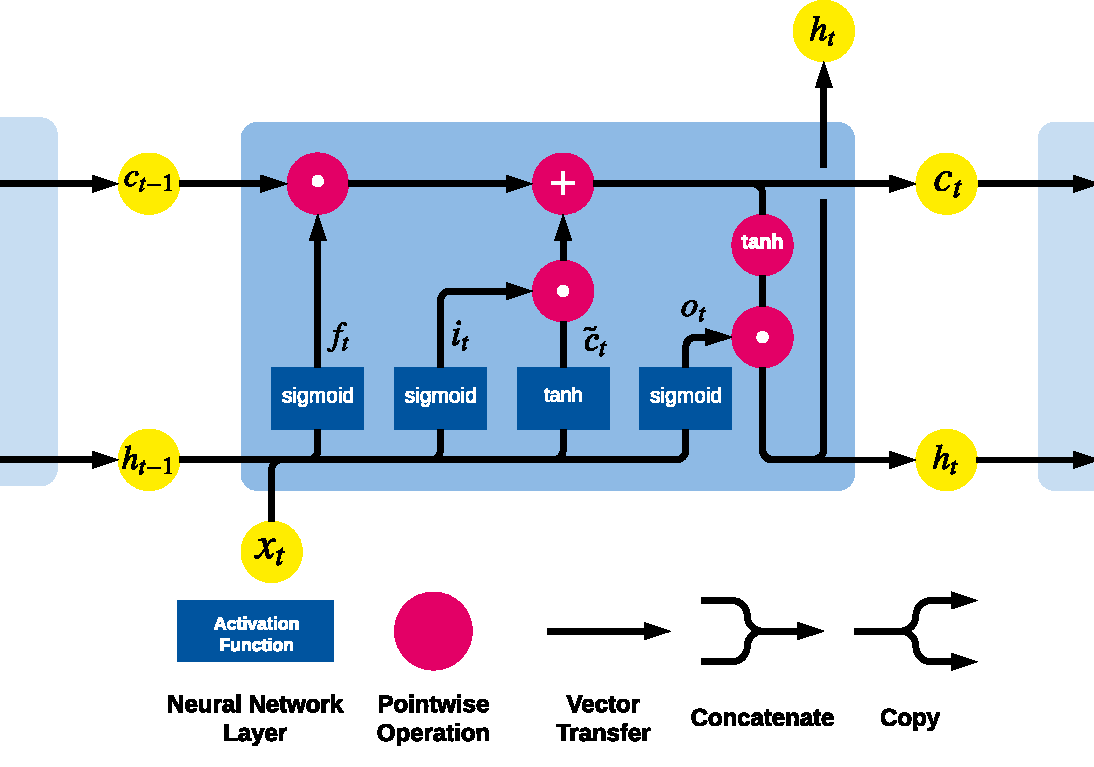
\includegraphics[width=0.9\textwidth]{figures/lstm-module}
	\caption[Structure of an LSTM module]{LSTM module with four sublayers that manipulate the cell state and compute the module's output. The graphic is adapted from \cite{lstm-blog}.}
	\label{fig:lstm-module}
\end{figure}

Recurrent neural networks extend traditional feedforward networks with backfeeding connections between hidden layers.
This enables the network to keep a state across inputs and allows the neural network to process arbitrarily long sequences of input data while learning temporal dependencies.

In LTSM networks the layers are replaced by more complex LSTM modules, where each module contains four different sublayers.
The architecture of a single LSTM module is shown in Figure \ref{fig:lstm-module}.
The module uses as input the state $\vec{c}_{t-1}$ and the hidden output $\vec{h}_{t-1}$ of the module in the previous time step as well as the output of the previous layer $\vec{x}_t$ to compute a new cell state $\vec{c}_{t}$ and a hidden output $\vec{h}_{t}$.

The input vector $\vec{x}_t$ is concatenated with the previous hidden output $\vec{h}_{t-1}$ and transferred to four neural network layers, which are designed to decide what part of the cell state will remain (forget gate $\vec{f}_t$), how it is updated (update gate $\vec{i}_t$ and $\vec{\tilde{c}}_t$) and what the output of the layer will be (output gate $\vec{o}_t$ leading to $\vec{h}_t$ considering the updated cell state $\vec{c_t}$).
The sublayer apply $\text{sigmoid}(x) = \frac{1}{1+\exp({-x})}$ or $\tanh(x) = \frac{\exp({x}) - \exp({-x})}{\exp({x}) + \exp({-x})}$ activation functions elementwise to vectors, leading to the following equations:
\begin{align*}
\vec{f}_t & = \text{sigmoid}(\vec{W}_f \cdot (\vec{h}_{t-1}, \vec{x}_t) + \vec{b}_f) \\
\vec{i}_t & =  \text{sigmoid} (\vec{W}_i \cdot (\vec{h}_{t-1}, \vec{x}_t) + \vec{b}_i) \\
\vec{\tilde{c}}_t & = \tanh (\vec{W}_c \cdot (\vec{h}_{t-1}, \vec{x}_t) + \vec{b}_c) \\
\vec{o}_t & =  \text{sigmoid} (\vec{W}_o \cdot (\vec{h}_{t-1}, \vec{x}_t) + \vec{b}_o)
\end{align*}
$\vec{W}_f$, $\vec{W}_i$, $\vec{W}_c$ and $\vec{W}_o$ are the sublayer's learned weights and $\vec{b}_f$, $\vec{b}_i$, $\vec{b}_c$ and $\vec{b}_o$ are the corresponding biases.
The new cell state $\vec{c}_t$ is then a combination of the old cell state $\vec{c}_{t-1}$ and the result of the update gate $\vec{\tilde{c}}_t$, where the layer computations $\vec{f}_t$ and $\vec{i}_t$ determine the proportions by a pointwise multiplication ($\odot$) with the cell states.
\begin{equation*}
	\vec{c}_t = f_t \odot \vec{c}_{t-1} + \vec{i}_t \odot \vec{\tilde{c}}_t
\end{equation*}
The result of the output gate $\vec{o}_t$ is pointwise multiplied with the tanh-activated new cell state to calculate the hidden output $\vec{h}_t$ of the module.
\begin{equation*}
	\vec{h}_t = \vec{o}_t \odot \tanh(\vec{c}_t )
\end{equation*}
LSTM networks are able to backpropagate a more stable error with this gating mechanism, such that these networks are much more capable of learning complex functions for sequences compared to standard recurrent neural networks.
As a machine learning model that naturally supports sequential data, LSTM networks are a suitable prediction model for processes.